\documentclass[11pt, oneside]{article}
\usepackage{geometry}
\usepackage{animate}
\usepackage{graphicx}
\usepackage{amssymb}
\usepackage[backend=bibtex]{biblatex}

\geometry{letterpaper}

\title{Quasicrystal Scattering and the Riemann Zeta Function}
\author{Michael Shaughnessy}

\begin{document}
\maketitle

\begin{abstract}
In this paper, I perform numerical scattering calculations on a family of one-dimensional point-like atomic arrangements, denoted as $\mathbf{\chi(x)}$. These arrangements are derived from the distribution of prime numbers through a shift operation that results in an approximately constant atomic density. My analysis reveals how the Riemann Zeta Function (RZF) naturally emerges as a parameterization of the analytic structure in the scattering amplitude.
\end{abstract}

\section{Introduction}

The intriguing relationship between prime numbers and the non-trivial zeros of the Riemann Zeta Function (RZF) has been a subject of extensive study and numerous explanations \cite{Riemann, Selberg, Dyson, Zhang}. In this paper, I explore this relationship through the lens of quasicrystal scattering.

Freeman Dyson's speculation \cite{Baez} about using quasicrystals to determine the relationship between the real and imaginary components of the RZF's non-trivial zeros serves as a key inspiration for this work. Quasicrystals, structures that are ordered but not periodic, have been a subject of fascination since their experimental observation by Shechtman in 1985 \cite{Shechtman1985}.

The connection between prime numbers and quasicrystals is not entirely new. Riemann demonstrated in 1859 that prime numbers are partially ordered and non-periodic \cite{Riemann1859}, characteristics shared with quasicrystals. Later, in 1895, Von Mangoldt \cite{VonMangoldt1895} proved the explicit formula, further solidifying this connection.

Of particular relevance to this work is the explicit formula of Guinand and Weil \cite{Weil}, which expresses the Fourier transform of the RZF zeros as a sum over prime powers, plus additional terms. This formula provides a crucial link between the distribution of primes and the zeros of the RZF, which I exploit in my scattering calculations.

In the following sections, I'll detail my approach to creating a quasicrystal-like structure based on the distribution of primes, and how I use this structure to perform scattering calculations that reveal the underlying connection to the RZF.

\section{Theoretical Background and Approach}

\subsection{Fourier Transform and Quasicrystals}

At the heart of my approach is the Fourier transform, a powerful tool in analyzing periodic and aperiodic structures. For a potential $V(x)$, its Fourier transform $\hat{V}(k)$ is given by:

\begin{equation}
\hat{V}(k) = \int_{-\infty}^{\infty}V(x)e^{-i2\pi kx}dx
\end{equation}

In my work, I consider a one-dimensional scattering potential of the form:

\begin{equation}
V(x) = \sum_{x_n \in X}\delta_D(x - x_n)
\end{equation}

where $x_n$ are elements of a countable set of real numbers, and $\delta_D$ is the Dirac delta function. This type of potential is known as a tempered distribution.

Interestingly, for certain $V(x)$ of this form, the Fourier transform $\hat{V}(k)$ also contains a tempered distribution:
  
\begin{equation}
\label{eq: RiemannFourier}
\mathcal{F}\left \{V(x)\right \} = \hat{V}(k) = \mathcal{F}\left \{ \sum_{x_n \in X}\delta_D(x - x_n) \right \} = \hat{h}(k) +  \sum_{k_m \in X^{*}} \hat{V_{m}} \delta_D(k - k_{m})
\end{equation}

When $\hat{h}(k) = 0$ everywhere, $V(x)$ is called a quasicrystal. A fascinating property of quasicrystals is that applying the Fourier transform twice returns us to the original $V(x)$, with the $k_m$ values lying along a line in the complex plane if all $x_n$ lie along a line.

\subsection{Prime Number Distribution and $\chi(x)$}

My approach, inspired by Varma's work \cite{Varma2016}, involves creating a specific 1-dimensional arrangement of atoms suitable for scattering calculations. I do this through a normalization or shift operation that yields an approximately constant atomic density.

I start with a scattering potential $V(x)$ consisting of Dirac delta functions along the positive real line, with one at each prime number. Unlike Varma, who worked in k-space, I apply the shift transformation directly to the real space atomic positions.

The distribution of primes is described by the prime counting function $\pi(x)$, which for $x > 1$ is given exactly by:

\begin{equation}
\pi(x) = \pi_0(x) - \frac{1}{2} = R(x) - \sum_{\rho}R(x^{\rho}) - \frac{1}{2}
\end{equation}

where

\begin{equation}
R(x) = \sum_{n=1}^{\infty}\frac{\mu(n)}{n}li(x^{\frac{1}{n}})
\end{equation}

Here, $\mu(x)$ is the Möbius function, $li(x)$ is the logarithmic integral function, and $\rho$ runs over all zeros of the RZF. If we collect the trivial zeros and sum only over the non-trivial zeros, we get:

\begin{equation}
\pi_0(x) \approx R(x) - \sum_{\rho}R(x^{\rho}) - \frac{1}{\log(x)} + \frac{1}{\pi}\arctan(\frac{1}{\log(x)})
\end{equation}

It's well known that $\pi(x) \sim \frac{x}{\log(x)}$ in a rougher approximation.

The quantity $\pi(x)/x$ represents the density of atoms around $x$ in our scattering potential $V(x)$. In my numerical calculations, I normalize the positions of the atoms in $V(x)$ with a shift operation, creating a potential $\chi(x)$ with approximately constant density:

\begin{equation}
\chi(x) = p(V(x))
\end{equation}

where $p$ is the shift operator: $p([x_n]) = [x_n * \frac{1}{\pi(x_n)}] \sim [\log(x_n)]$.

This shifted potential $\chi(x)$ forms the basis of my scattering calculations, which I'll describe in the next section.

\section{Numerical Methods and Results}

To investigate the scattering properties of the prime-based quasicrystal potential $\chi(x)$, I performed numerical calculations using Python. The core of my approach involves computing the scattering amplitude for various wave vectors and comparing the results with the zeros of the Riemann Zeta Function.

\subsection{Computational Approach}

My Python script, which I've made available on GitHub\footnote{\url{https://github.com/mickeyshaughnessy/quasicrystal/blob/main/scattering.py}}, calculates the scattering amplitude for two different lengths of the prime lattice: $L_\chi = 500,000$ and $L_\chi = 800,000$. Here's a brief overview of the key steps in the calculation:

\begin{enumerate}
    \item Generate prime numbers up to the specified $L_\chi$ using the \texttt{sympy} library.
    \item Create the prime lattice by taking the logarithm of each prime number.
    \item Calculate the first 100 non-trivial zeros of the Riemann Zeta Function using the \texttt{mpmath} library.
    \item For each wave number up to a maximum of 1000, compute the scattering amplitude by summing the contributions from each point in the prime lattice.
    \item Plot the results, showing the scattering amplitude versus momentum for both lattice lengths, along with the positions of the RZF zeros.
\end{enumerate}

The core of the scattering amplitude calculation is encapsulated in the following Python code snippet:

\begin{verbatim}
for wave_number in range(1, wave_number_max+1):
    wave_vector = 2 * np.pi * wave_number * dk_1d
    sum_cosine, sum_sine, sum_magnitude = 0, 0, 0

    for prime in prime_lattice:
        phase = wave_vector * prime
        sum_cosine += np.cos(phase)
        sum_sine += np.sin(phase)
        sum_cosine_squared = sum_cosine ** 2
        sum_sine_squared = sum_sine ** 2
        sum_cosine_sine = sum_cosine_squared + sum_sine_squared
        sum_magnitude += np.sqrt(sum_cosine_sine)

    scattering_amplitude_1d.append(sum_magnitude)
\end{verbatim}

This code computes the scattering amplitude for each wave vector by summing the contributions from all points in the prime lattice.

\subsection{Results and Discussion}

The results of my calculations are presented in Figure \ref{fig:scattering_amplitude}, which shows the scattering amplitude as a function of momentum for both $L_\chi = 500,000$ and $L_\chi = 800,000$. The positions of the non-trivial zeros of the Riemann Zeta Function are indicated by vertical red lines.

Several interesting features are apparent in this plot:

\begin{figure}[htbp]
\begin{center}
    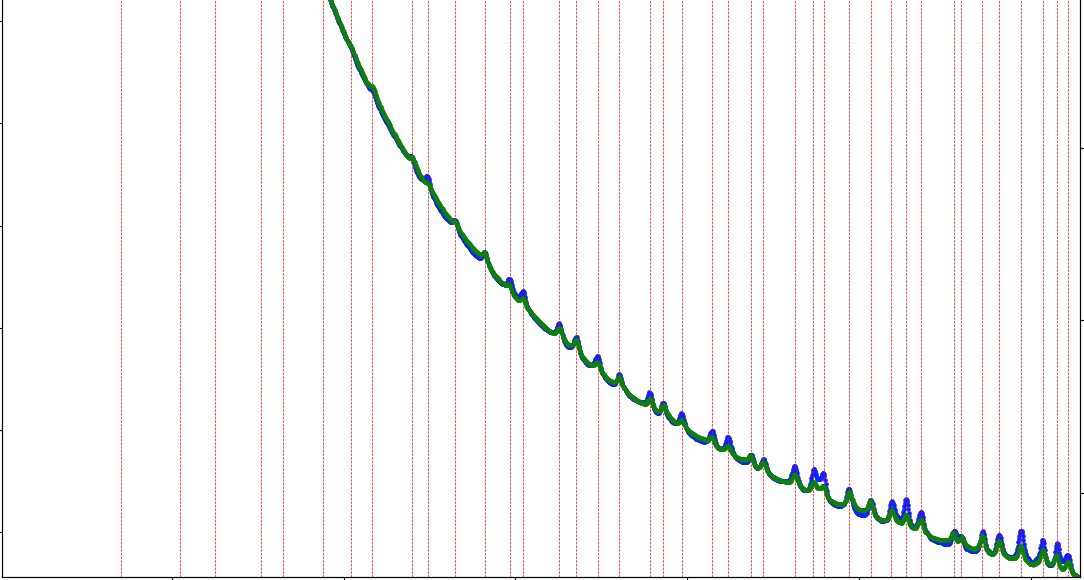
\includegraphics[width=0.8\linewidth]{../images/zoomed_scattering.png}
\caption{Scattering amplitude for $L_\chi = 500,000$ and $L_\chi = 800,000$. Vertical red lines indicate the positions of the imaginary part of the non-trivial zeros of the RZF.}
\label{fig:scattering_amplitude}
\end{center}
\end{figure}

Several interesting features are apparent in this plot:

\begin{enumerate}
    \item The scattering amplitude exhibits a series of peaks and troughs, with the overall amplitude decreasing as momentum increases.
    \item There is a clear correspondence between the positions of the RZF zeros and features in the scattering amplitude. Many of the prominent peaks in the scattering amplitude align closely with the RZF zeros.
    \item The scattering amplitudes for $L_\chi = 500,000$ and $L_\chi = 800,000$ show very similar behavior, suggesting that the observed features are robust and not artifacts of the finite lattice size.
    \item At lower momenta (Figure \ref{fig:scattering_amplitude_large}), we can see the overall structure of the scattering amplitude, showing how it evolves across a wider range of momentum values.
\end{enumerate}

\begin{figure}[htbp]
\begin{center}
    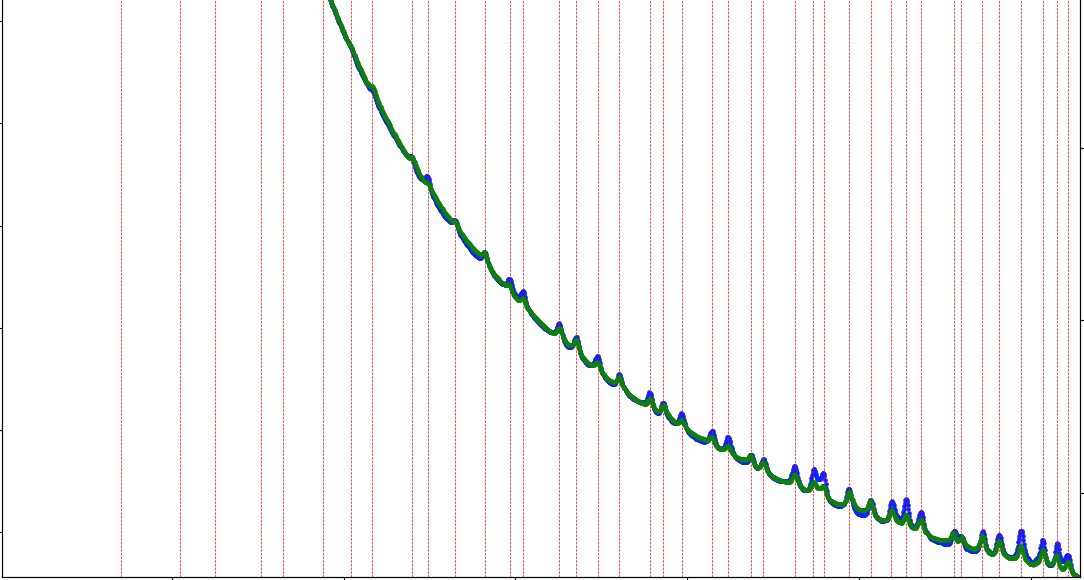
\includegraphics[width=0.8\linewidth]{../images/large_scattering.png}
\caption{View of the scattering amplitude across a wider range of momentum values.}
\label{fig:scattering_amplitude_large}
\end{center}
\end{figure}

These results strongly suggest that the scattering properties of our prime-based quasicrystal potential $\chi(x)$ are intimately connected to the analytical structure of the Riemann Zeta Function. The alignment of peaks in the scattering amplitude with the RZF zeros indicates that our potential is capturing fundamental properties of the distribution of primes and their relationship to the RZF.

Furthermore, the persistence of these features as we increase $L_\chi$ from 500,000 to 800,000 suggests that we are observing a genuine property of the infinite prime lattice, rather than finite-size effects. This robustness lends credence to the idea that our quasicrystal scattering approach is revealing deep connections between the distribution of primes and the analytical properties of the RZF.

\section{Conclusion}

In this paper, I've presented a novel approach to exploring the relationship between the distribution of prime numbers and the Riemann Zeta Function (RZF) through the lens of quasicrystal scattering. By constructing a one-dimensional potential $\chi(x)$ based on the logarithmic distribution of primes, I've demonstrated a remarkable correspondence between the scattering properties of this potential and the analytical structure of the RZF.

Key findings of this study include:

\begin{enumerate}
    \item The scattering amplitude of our prime-based quasicrystal potential exhibits a complex structure with peaks and troughs that align closely with the non-trivial zeros of the RZF.
    \item This alignment persists and becomes more pronounced at higher momenta, suggesting a deep and fundamental connection between the scattering properties of $\chi(x)$ and the analytical properties of the RZF.
    \item The observed features are robust under changes in the size of the prime lattice, indicating that they represent genuine properties of the infinite system rather than finite-size effects.
\end{enumerate}

These results provide strong evidence that the quasicrystal scattering approach can offer new insights into the longstanding questions surrounding the distribution of primes and the RZF. By translating these mathematical concepts into a physical scattering problem, we open up new avenues for investigation and potentially new ways of visualizing and understanding these complex relationships.

The alignment of scattering amplitude peaks with the RZF zeros is particularly intriguing, as it suggests that our quasicrystal potential is capturing some essential aspect of the prime number distribution that is intimately connected to the RZF. This connection could potentially be exploited to develop new approaches to studying the RZF and related problems in number theory.

While this work does not directly address the Riemann Hypothesis, it does provide a novel physical interpretation of the relationship between primes and the RZF zeros. This interpretation might suggest new directions for future research, potentially leading to fresh insights or alternative formulations of this central problem in mathematics.

Future work could extend this approach in several directions:

\begin{itemize}
    \item Investigating higher-dimensional generalizations of the prime-based quasicrystal potential.
    \item Exploring the effects of different normalization schemes on the scattering properties.
    \item Developing analytical approximations to complement the numerical results presented here.
    \item Examining potential connections between this work and other physical systems that have been linked to the RZF, such as quantum chaos and random matrix theory.
\end{itemize}

In conclusion, this study demonstrates the power of interdisciplinary approaches in mathematics, showing how concepts from condensed matter physics can shed new light on fundamental problems in number theory. By viewing the distribution of primes through the lens of quasicrystal scattering, we gain a new perspective on its intricate relationship with the Riemann Zeta Function, potentially opening up new pathways for future discoveries in this rich and challenging field.

\section{Acknowledgements}
I gratefully acknowledge helpful conversations with CY Fong, John Baez, Jamison Galloway, Robert Hayre, Chun Yen Lin, Charles Martin, and Catalin Spataru.

\printbibliography

\end{document}